\newpage 
\section{Google File System (GFS)}
\label{sec:gfs}

\noindent
Its 2003 and a research paper by Sanjay Ghemawat, Howard Gobioff, and Shun-Tak Leung, lay out
what would become the Google File System (GFS). In the early 2000s,
Google rapidly expanded its workload, scaling to support services like,
web search, indexing, and data analytics. Traditional file 
systems were not suited for their needs. Hence, GFS was designed for the following (Below you may find the GFS paper
(\href{https://static.googleusercontent.com/media/research.google.com/en//archive/gfs-sosp2003.pdf}{Original Paper}):

\begin{Def}[Design Goals of GFS]
  
  \textbf{Google File System (GFS)} is a distributed file system, which aims to have:
  \begin{itemize}
    \item \textbf{Massive scalability:} Store vast amount of data across thousands of inexpensive commodity servers.
    \item \textbf{High availability:} Tolerant to \underline{frequent} component failures \textbf{(replication needed)}.
    \item \textbf{High throughput:} Optimize for large data-streams of concurrent sequential reads and a majority of append-only writes.
  \end{itemize}

  \noindent
  \textbf{Consistency Model:} \underline{Weak consistency model} for improved performance.
\end{Def}

\vspace{1em}
\begin{figure}[h]
  \centering
  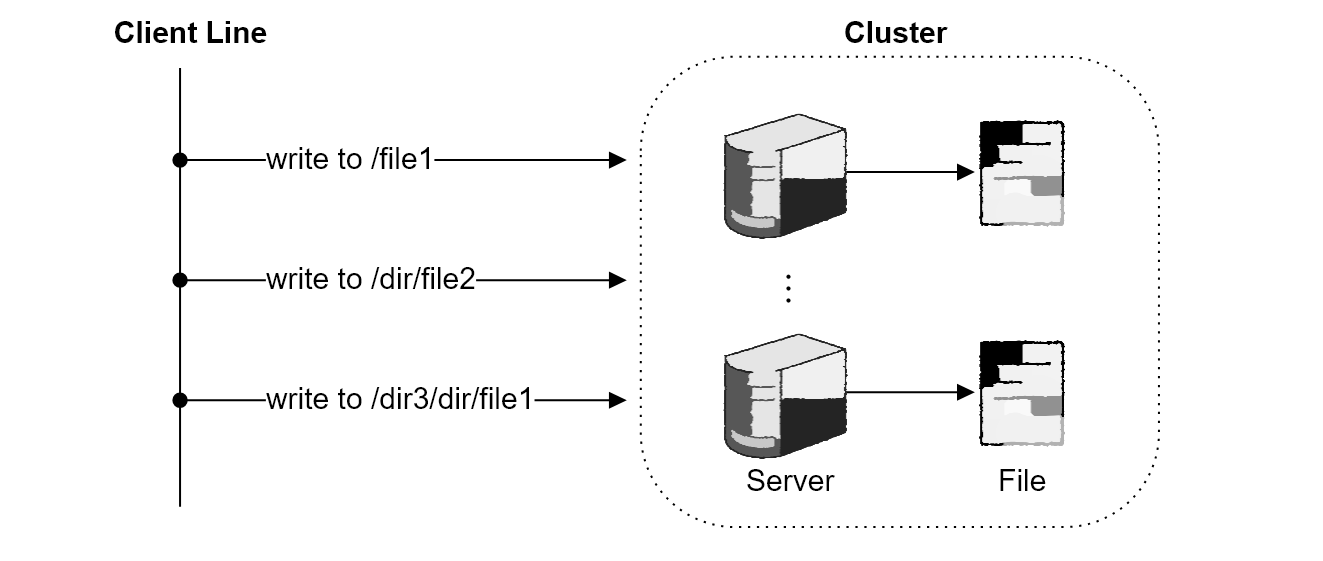
\includegraphics[width=\textwidth]{Sections/gfs/gfs.png}
  \caption{A high-level sketch of the Google File System (GFS) architecture.}
  \label{fig:gfs-architecture}

\end{figure}

\vspace{1em}
\noindent
\textbf{Note}: This is important as Google at the time was using cheap commodity hardware, which was prone to failure.

\newpage 

\noindent
The following details how files are stored in GFS:

\begin{Def}[File Chunking]

  Files in GFS are divided into \underline{fixed-size chunks} of 64MB.
  Each chunk is stored in a \textbf{chunk server}, identified by a unique 64 bit ID called a \textbf{chunk handle}.

  \underline{To ensure fault tolerance,} each chunk is \textbf{replicated} at least $N$ times across different chunk servers (Typically $N=3$).
\end{Def}

\begin{figure}[h]
  \centering
  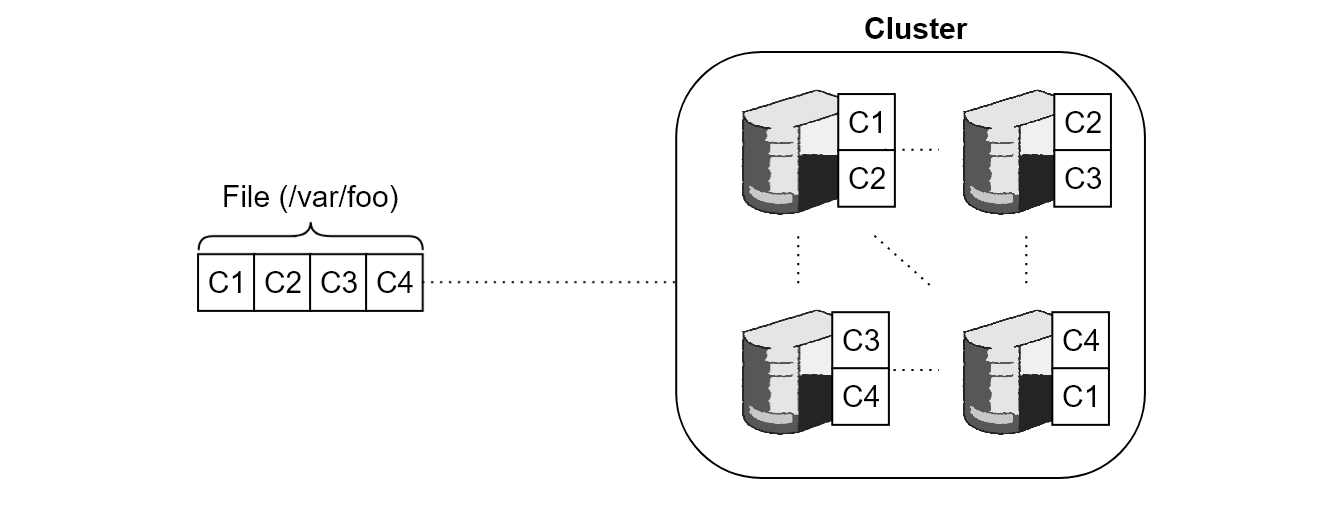
\includegraphics[width=\textwidth]{Sections/gfs/chunk.png}
  \caption{Simplified view of chunking in GFS, where a file is divided into 4 chunks (C1--C4), replicated twice across different servers.}
  \label{fig:gfs-chunking}
\end{figure}


\noindent
We decide to store metadata on a dedicated server to act as our coordinator.
\begin{Def}[Metadata Management]

  The GFS \textbf{master} serves \textbf{one cluster}, storing the following metadata in memory:
  \begin{itemize}
    \item \textbf{File \& Chunk Namespaces:} Hierarchical directory tree of files and the global chunk-ID namespace.
    \item \textbf{File$\to$Chunk Mapping:} For each file, the ordered list of chunk handles.
    \item \textbf{Chunk Replica Locations:} Connecting chunk handles to their chunk servers holding its replicas via [IP:port].
    \item \textbf{Access Control Information:} File permissions and ownership attributes.
  \end{itemize}
  
  \noindent
  In particular, mappings are persisted via an operation log. 
  Chunk locations are reconstructed by polling chunk servers at startup or when they join.
\end{Def}




\newpage

\noindent
Now to discuss how client's read data from GFS:
\begin{Def}[Client Interaction]

  \textbf{Clients} interact with GFS via a \underline{two-step process}:
  \begin{itemize}
    \item \textbf{Metadata Operations:} Clients query the master with the (file name, chunk index), receiving the chunk handle and its replica locations.
    \item \textbf{Data Operations:} The client caches such information and then directly communicate with the chunk servers.
  \end{itemize}
\end{Def}

\begin{figure}[h]
  \centering
  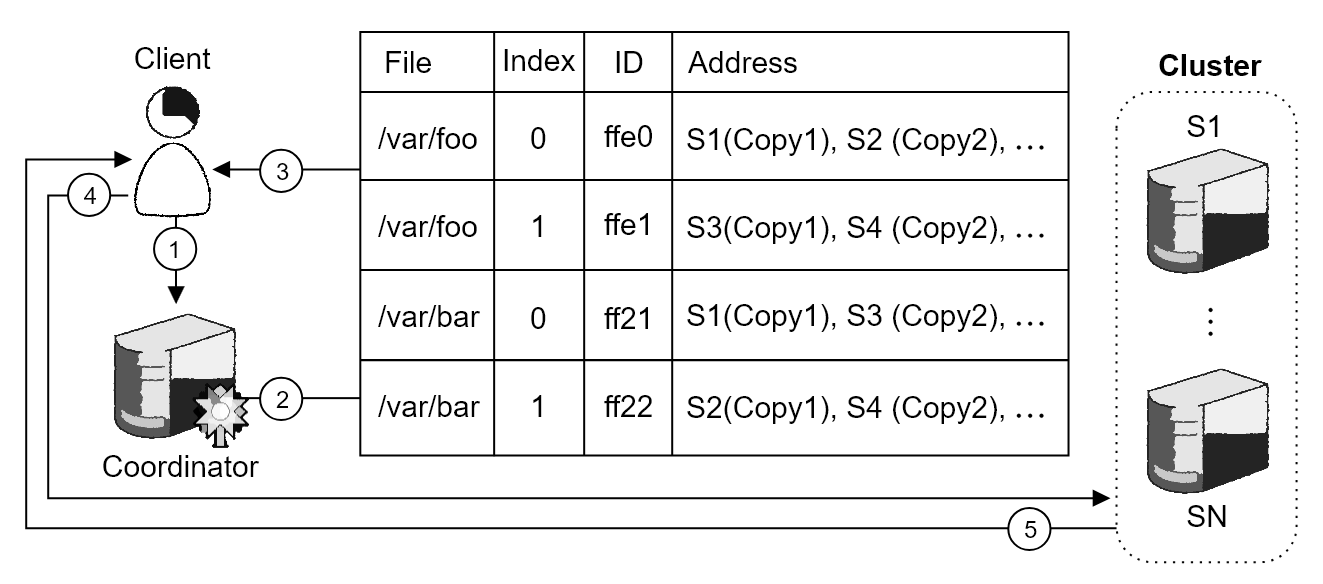
\includegraphics[width=\textwidth]{Sections/gfs/interaction.png}
  \caption{A Simplified view of client interaction with GFS. (1) Client sends a request to the master for metadata. (2) The master finds the chunk handle and its replica locations. 
  (3) The master returns the chunk handle and replica locations to the client. (4) The client sends a request to the chunk server for data. (5) The chunk server returns the data to the client.}
  \label{fig:gfs-client}
\end{figure}
    
\noindent
In our case we have specific needs that allow staleness to be tolerated:
\begin{Def}[GFS -- Stale Reads are Allowed]

  Given the application of GFS's workload, it is acceptable to have stale reads. This greatly improves performance, as we don't have to 
  have additional round trips to ensure the data is up to date. 

  For example, we may be gathering analytics which improve search results. Retrieving stale data doesn't break the system. When the latest data does arrive, we notice improved performance.
\end{Def}
\newpage 
\noindent
The client reads and writes data in two slightly different ways:
\begin{Def}[Read and Write Routines]

  \textbf{Reads:} The clients retrieves a server location from the master, reading directly from them.
  \textbf{Writes:} Follow a \underline{three-step process}:
  \begin{itemize}
    \item \textbf{Metadata Retrieval:} Clients query the master with the (file name, chunk index), receiving a list of replica locations. The master chooses one server to be the \textbf{primary replica}, granting it a \textbf{lease}, which defines the time period such server may act as the primary replica (typically 60s).
    \item \textbf{Data Transfer:} From the list of replicas, the client sends the data to the \textbf{closest replica} (not necessarily the primary replica). Such replica propagates the data to the next closest server, and so forth.
    \item \textbf{Commit Phase:} The client sends a \textbf{commit} request to the primary replica, which then notifies the other replicas to apply the changes. The primary replica then sends an \textbf{ACK} to the client.
  \end{itemize}
\end{Def}

\noindent
In particular, the primary server follows a specific routine:
\begin{Def}[Primary Server Routine]

  \label{def:primary}
  The \textbf{primary} replica orchestrates concurrent writes with strict per-mutation ordering:
  \begin{itemize}
    \item \textbf{Lease Validation:} Upon each \texttt{WriteChunk} RPC, check that the primary's lease (granted by the master) is still valid. If it has expired, reject the request so the client can \textbf{refresh} metadata.
    \item \textbf{Replica-log ACKs:} The client waits for all replicas to ACK that the log has been replicated. Then it tells the primary to commit.
    \item \textbf{Per-Mutation Sequencing \& Serialization:} Each incoming write is assigned a consecutive sequence number (possibly from multiple clients), which will be applied in sequential order.
    \item \textbf{Commit and Reply:} On command, the primary server applies the mutation in serial order, telling the secondaries to do the same; \textbf{However}, 
    the primary sends the ACK to the client immediately even before any replicas even acknowledge the commit.
    
    \quad This means \textbf{stale data} may be latent in the system. Though, our master will eventually catch this, and re-replicate the data.
    \item \textbf{Error Handling:} If any secondary fails to replicate the log in time (not the apply phase), abort the mutation, notify the client, and rely on the client's retry logic.
  \end{itemize}
\end{Def}

\newpage 
\noindent
We illustrate the write process in the figure below:

\begin{figure}[h]
  \centering
  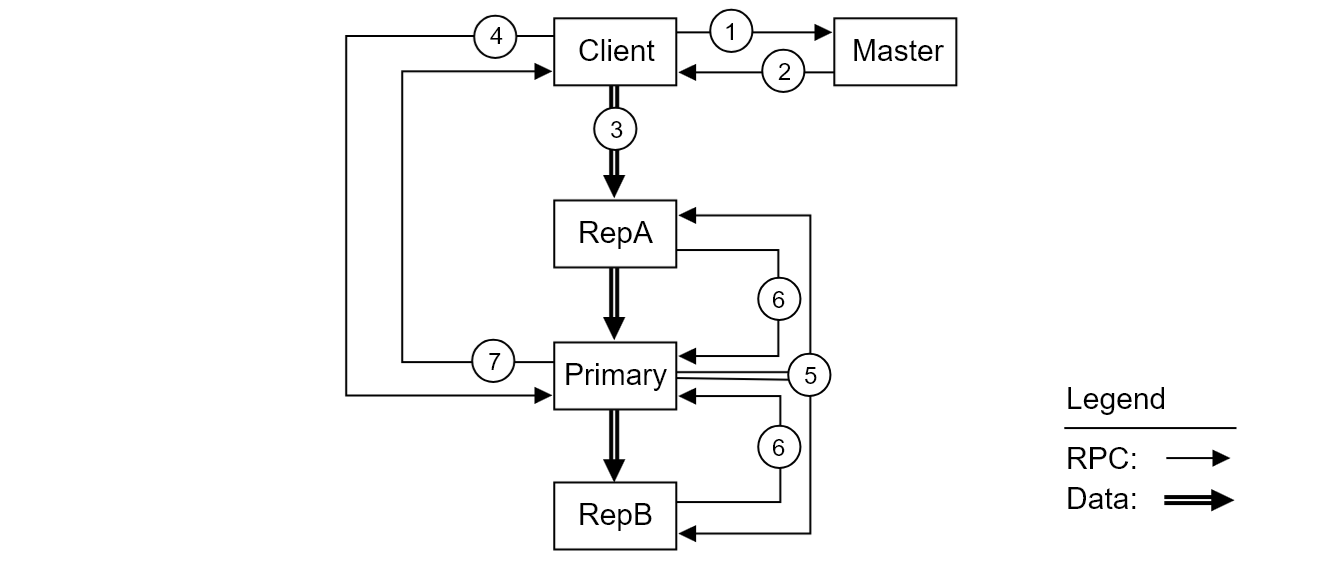
\includegraphics[width=\textwidth]{Sections/gfs/write.png}
  \caption{A Simplified view of the write process in GFS. (1) Client sends a request to the master for metadata. (2) The master finds the chunk handle and its replica locations. 
  (3) The client sends a request to the closest replica who propagates it through the network. (4) After receiving ACKs from all replicas, the client sends a commit request to the primary replica. (5) The primary replica sends a commit request to all replicas. (6) The replicas send ACKs back to the primary replica. (7) The primary replica sends an ACK back to the client.}
  \label{fig:gfs-write}
\end{figure}

\noindent
Now we need to ensure there are $N$ copies of a chunk at all times:
\begin{Def}[Chunkserver Heartbeat Routine]
  \textbf{Chunkservers} send periodic \textbf{HeartBeat} RPCs to the master, conveying:
  \begin{itemize}
    \item \textbf{Held Chunk Handles \& Versions:} The set of chunk IDs stored locally along with each chunk's current version, \underline{so the master can detect \textbf{missing or stale replicas}.}
    \item \textbf{Lease Extension Requests:} Any primary replicas include lease-renewal requests for the chunks they lead.
  \end{itemize}
  \noindent
  The master's response piggy-backed on the heartbeat (reply to such heartbeat) may grant new leases or issue commands (e.g.\ initiate re-replication). If a chunk server's heartbeat is not received within a timeout, the master marks it dead and schedules re-replication to restore $N$ live replicas per chunk.
\end{Def}

\newpage 
\noindent
The master handles persistent state and snapshots for log reduction in the following way:
\begin{Def}[Master Checkpoint \& Operation-Log Routine]

  The \textbf{master} persists its metadata through two complementary mechanisms:
  \begin{itemize}
    \item \textbf{Operation Log:} An append-only record of every metadata-mutating request (e.g.\ file/ directory creation, chunk allocation).  Each entry is synchronously written to the master's local disk and replicated to remote machines.
    \item \textbf{Periodic Checkpoints:} In a background thread, the master periodically snapshots its entire in-memory state (file and chunk namespaces plus file$\to$chunk mappings), writes the checkpoint to disk, and safely truncates the operation log up to that point.
  \end{itemize}
  \noindent
  On startup (or after a crash), the master loads the latest checkpoint and then replays any subsequent operations from the log to reconstruct its full metadata state.
\end{Def}
\noindent
In short, the master must keep record of any critical changes to the metadata, and sufficiently back it up to ensure it can recover. Though,
having a single master is a bottleneck. Hence, we keep a replica in the background:
\begin{Def}[Shadow Master]

  A \textbf{shadow master} is a standby replica of the GFS master that provides high availability:
  \begin{itemize}
    \item \textbf{Operation-Log Mirroring:} Maintains a copy of the master's operation log, replicated remotely.
    \item \textbf{State Replay:} Continuously \textbf{replays} (applies) logged operations to keep its in-memory metadata (namespaces and file→chunk mappings) nearly up to date.
    \item \textbf{Read-Only Serving:} Can answer client metadata queries (e.g.\ lookups) in a read-only fashion, offloading the active master.
    \item \textbf{Failover Ready:} On active-master failure, a simple DNS switch (switching the network pointer to the master) promotes the shadow to become the new active master.
    \item \textbf{Eventual Consistency:} May lag slightly behind the active master due to asynchronous log replication and replay.
  \end{itemize}
\end{Def}

\newpage 
\noindent
Though we must point out:
\begin{theo}[Non-Atomicity and Non-Serializability Across Chunk Boundaries]

  In GFS, writes that span multiple chunks are neither atomic nor globally serializable. Concretely, there exist two concurrent write operations $W_1$ and $W_2$ and chunk indices $i\neq j$,
  such that the primary for chunk $i$ orders $W_1$ before $W_2$, while the primary for chunk $j$ orders $W_2$ before $W_1$.\\

  \noindent
  \textbf{However}, concurrent writes are atomic and serializable \textbf{within a single chunk}.
\end{theo}
  
\noindent
To point out, and emphasize:
\begin{Def}[One Primary for each Chunk]

  In GFS, each chunk is assigned exactly one \textbf{primary} replica by the master via a lease.
\end{Def}

\vspace{-.3em}
\begin{figure}[h]
  \centering
  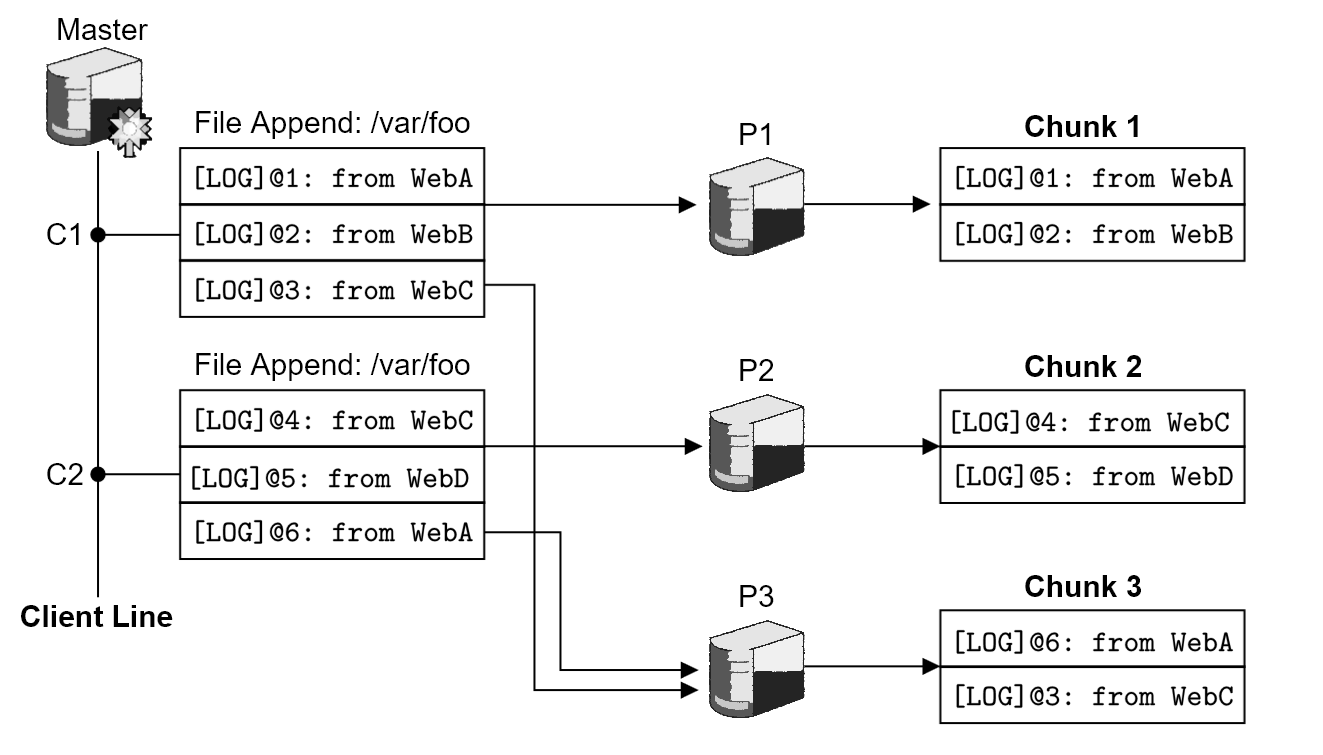
\includegraphics[width=\textwidth]{Sections/gfs/atomic.png}
  \caption{GFS record-append across chunk boundaries (client$\to$master$\to$client$\to$primary). 
  Each chunk holds up to two log records. Clients $C_1,C_2$ issue appends \texttt{@1}--\texttt{@6}. Under primary $P_1$ (chunk 1), \texttt{@1},\texttt{@2} succeed while the rest are rejected. Each client then re-queries the master and retries on primary $P_2$ (chunk 2), where \texttt{@4},\texttt{@5} succeed but \texttt{@3},\texttt{@6} are rejected. A final refresh to primary $P_3$ (chunk 3)
  accepts \texttt{@6},\texttt{@3} in arrival order, illustrating that independent primaries can impose different orders, and that multi-chunk appends are non-atomic and non-serializable.}

  \label{fig:gfs-primary}
\end{figure}
    
\newpage 

\noindent
Below we summarize the key points of GFS through an illustration:
\begin{figure}[h]
  \centering
  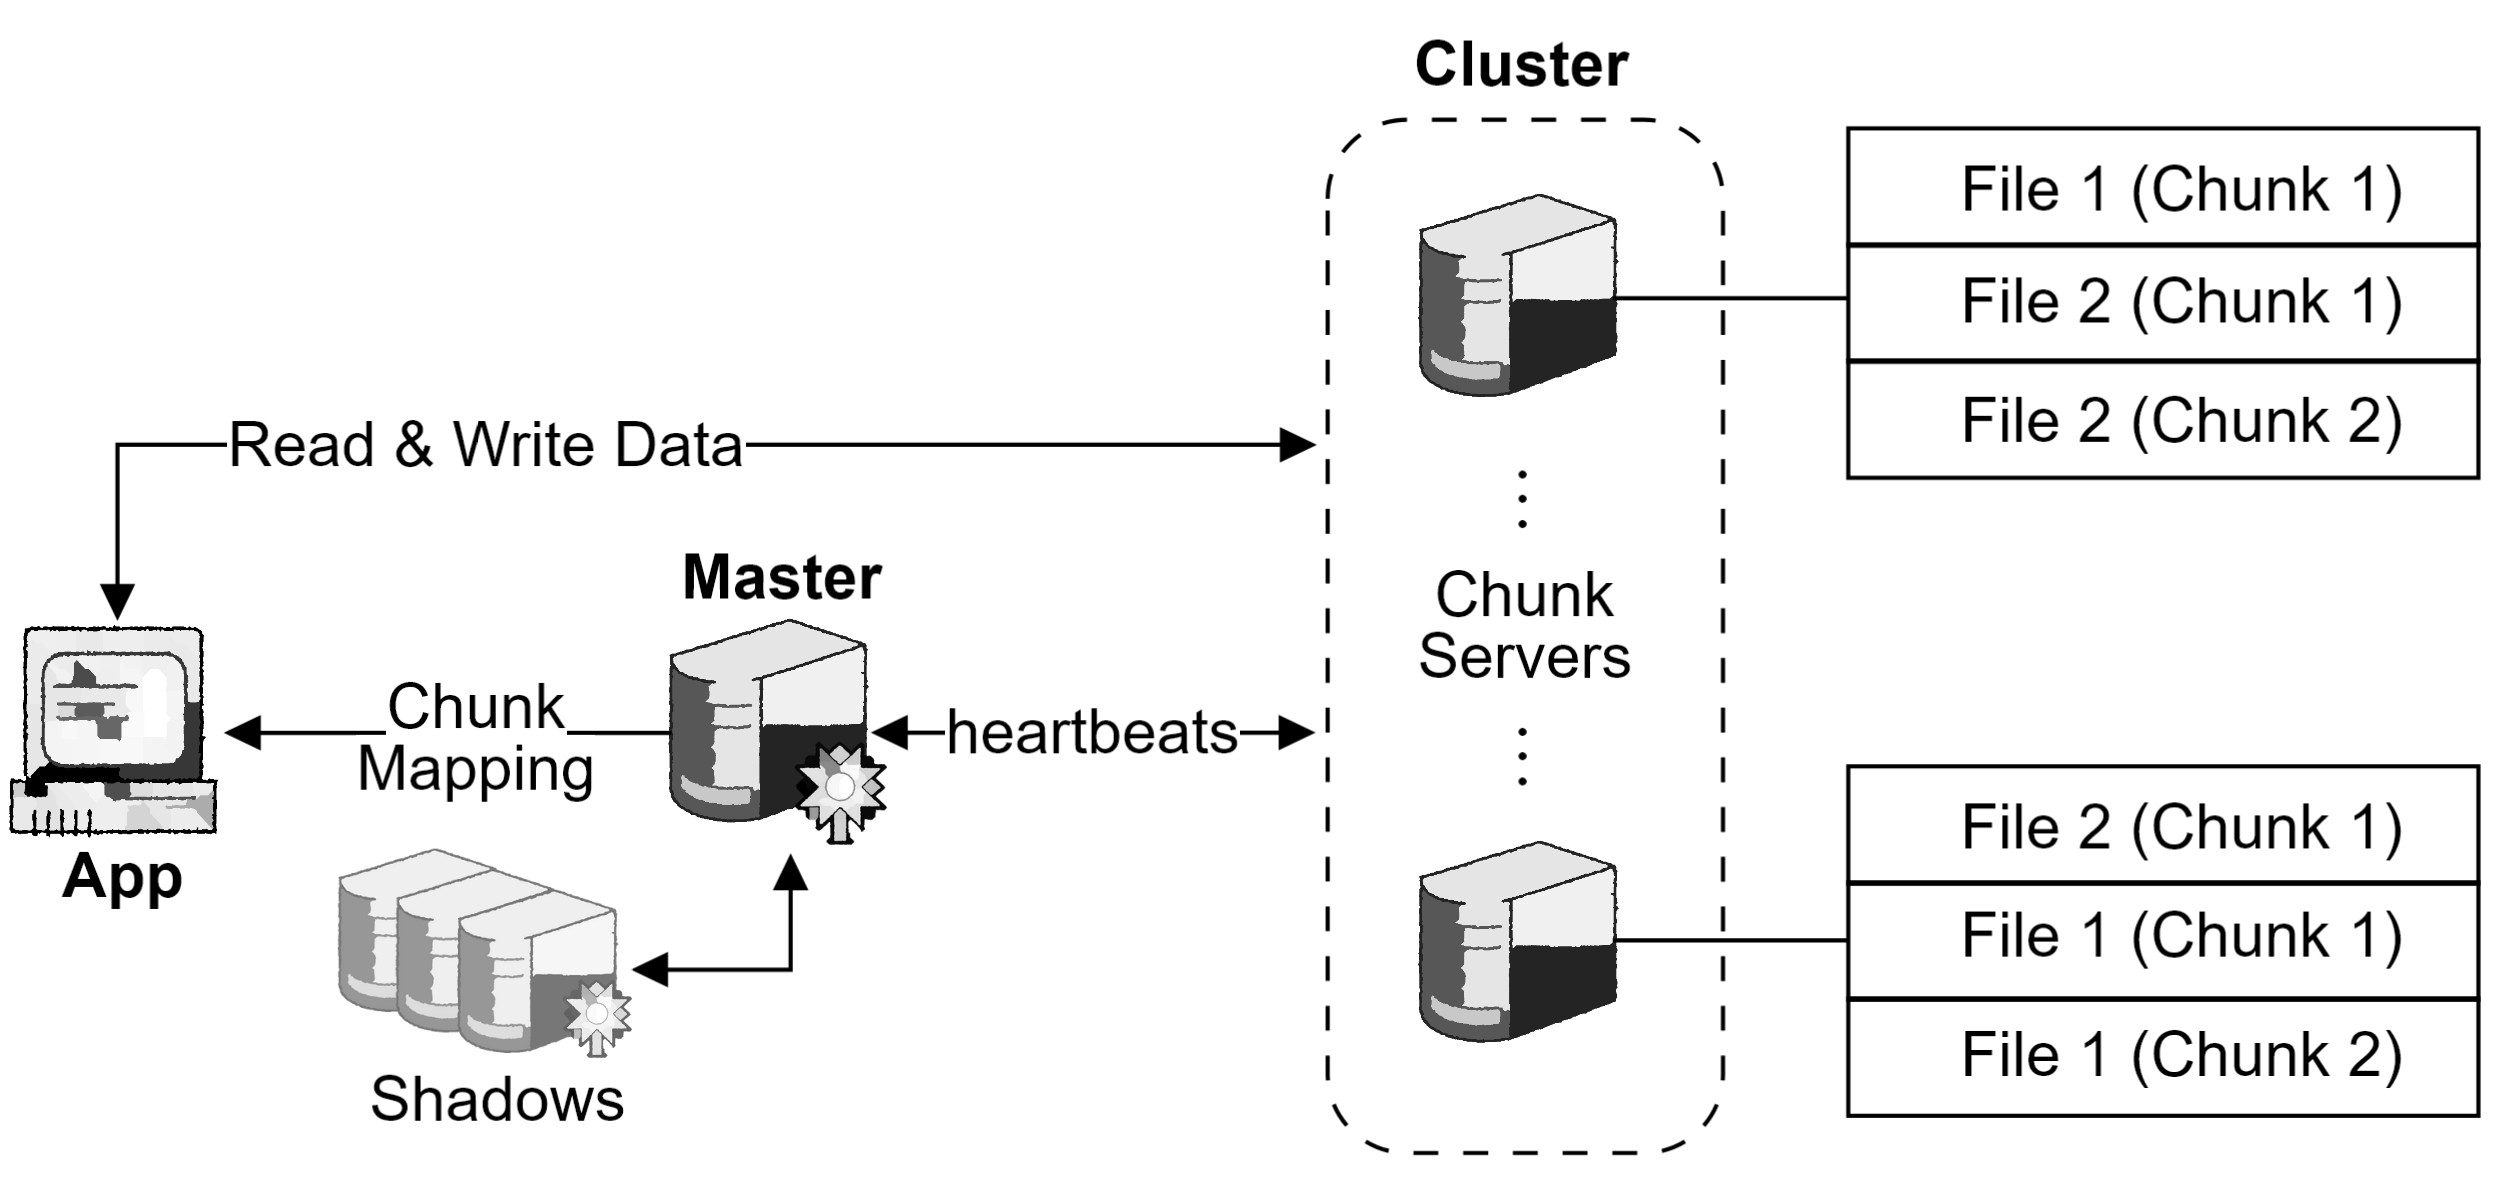
\includegraphics[width=\textwidth]{Sections/gfs/high.png}
  \caption{High-level GFS architecture. An application (\texttt{App}) first contacts the \textbf{master} to obtain file$\to$chunk mapping (via file name and chunk index), then directly reads from or writes to the appropriate \textbf{chunk servers}, 
  which store fixed-size, replicated chunks (e.g.\ chunks of File 1 and File 2) across the cluster. The master keeps all metadata in memory, persists mutating operations in an append-only operation log, and receives periodic \textbf{HeartBeat} RPCs from chunk servers to monitor 
  replica state and grant leases. \textbf{Shadow masters} asynchronously replay the operation log to maintain a nearly up-to-date, read-only metadata copy for load-sharing and fast failover.}
  \label{fig:gfs-summary}
\end{figure}


